\chapter{UML Diagrams}
\label{app:uml}

This appendix contains complete UML diagrams for the system architecture.

\section{Use Case Diagram}

\begin{figure}[H]
\centering
\begin{tikzpicture}[scale=0.8]
    % Actors
    \node[draw, ellipse] (user) at (-3,0) {Hotspot Owner};
    \node[draw, ellipse] (client) at (-3,-4) {Connected Client};
    
    % Use cases
    \node[draw, ellipse, minimum width=3cm] (activate) at (2,2) {Activate QoS};
    \node[draw, ellipse, minimum width=3cm] (deactivate) at (2,0) {Deactivate QoS};
    \node[draw, ellipse, minimum width=3cm] (assign) at (2,-2) {Assign Priority};
    \node[draw, ellipse, minimum width=3cm] (monitor) at (2,-4) {Monitor Traffic};
    \node[draw, ellipse, minimum width=3cm] (send) at (6,-4) {Send Traffic};
    
    % Associations
    \draw (user) -- (activate);
    \draw (user) -- (deactivate);
    \draw (user) -- (assign);
    \draw (user) -- (monitor);
    \draw (client) -- (send);
\end{tikzpicture}
\caption{Use Case Diagram}
\end{figure}

\section{Class Diagram}

\begin{figure}[H]
\centering
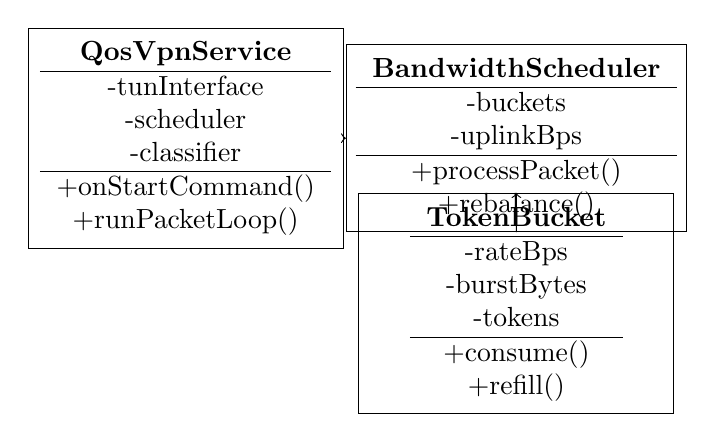
\begin{tikzpicture}[scale=0.7]
    % QosVpnService
    \node[draw, rectangle, minimum width=4cm, minimum height=2cm] (vpn) at (0,0) {
        \begin{tabular}{c}
            \textbf{QosVpnService} \\
            \hline
            -tunInterface \\
            -scheduler \\
            -classifier \\
            \hline
            +onStartCommand() \\
            +runPacketLoop()
        \end{tabular}
    };
    
    % BandwidthScheduler
    \node[draw, rectangle, minimum width=4cm, minimum height=2cm] (scheduler) at (6,0) {
        \begin{tabular}{c}
            \textbf{BandwidthScheduler} \\
            \hline
            -buckets \\
            -uplinkBps \\
            \hline
            +processPacket() \\
            +rebalance()
        \end{tabular}
    };
    
    % TokenBucket
    \node[draw, rectangle, minimum width=4cm, minimum height=2cm] (bucket) at (6,-3) {
        \begin{tabular}{c}
            \textbf{TokenBucket} \\
            \hline
            -rateBps \\
            -burstBytes \\
            -tokens \\
            \hline
            +consume() \\
            +refill()
        \end{tabular}
    };
    
    % Associations
    \draw[->] (vpn) -- (scheduler);
    \draw[->] (scheduler) -- (bucket);
\end{tikzpicture}
\caption{Class Diagram (Simplified)}
\end{figure}

\section{Sequence Diagram: Packet Processing}

\begin{figure}[H]
\centering
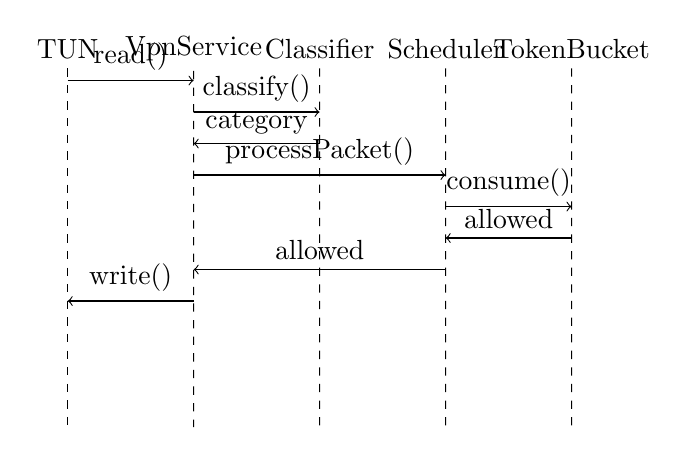
\begin{tikzpicture}[scale=0.8]
    % Lifelines
    \node (tun) at (0,0) {TUN};
    \node (vpn) at (2,0) {VpnService};
    \node (classifier) at (4,0) {Classifier};
    \node (scheduler) at (6,0) {Scheduler};
    \node (bucket) at (8,0) {TokenBucket};
    
    \draw[dashed] (tun) -- (0,-6);
    \draw[dashed] (vpn) -- (2,-6);
    \draw[dashed] (classifier) -- (4,-6);
    \draw[dashed] (scheduler) -- (6,-6);
    \draw[dashed] (bucket) -- (8,-6);
    
    % Messages
    \draw[->] (0,-0.5) -- (2,-0.5) node[midway, above] {read()};
    \draw[->] (2,-1) -- (4,-1) node[midway, above] {classify()};
    \draw[->] (4,-1.5) -- (2,-1.5) node[midway, above] {category};
    \draw[->] (2,-2) -- (6,-2) node[midway, above] {processPacket()};
    \draw[->] (6,-2.5) -- (8,-2.5) node[midway, above] {consume()};
    \draw[->] (8,-3) -- (6,-3) node[midway, above] {allowed};
    \draw[->] (6,-3.5) -- (2,-3.5) node[midway, above] {allowed};
    \draw[->] (2,-4) -- (0,-4) node[midway, above] {write()};
\end{tikzpicture}
\caption{Sequence Diagram: Packet Processing}
\end{figure}

\section{State Diagram: Token Bucket}

\begin{figure}[H]
\centering
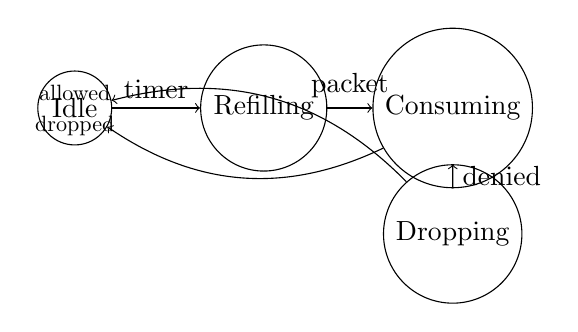
\begin{tikzpicture}[scale=0.8]
    \node[draw, circle] (idle) at (0,0) {Idle};
    \node[draw, circle] (refill) at (3,0) {Refilling};
    \node[draw, circle] (consume) at (6,0) {Consuming};
    \node[draw, circle] (drop) at (6,-2) {Dropping};
    
    \draw[->] (idle) -- (refill) node[midway, above] {timer};
    \draw[->] (refill) -- (consume) node[midway, above] {packet};
    \draw[->] (consume) to[bend left] (idle) node[midway, above] {allowed};
    \draw[->] (consume) -- (drop) node[midway, right] {denied};
    \draw[->] (drop) to[bend right] (idle) node[midway, below] {dropped};
\end{tikzpicture}
\caption{State Diagram: Token Bucket}
\end{figure}

\textit{(Complete UML diagrams including component diagram, deployment diagram, and activity diagrams available in project documentation)}
